\documentclass[a4paper,10pt]{article}

%page geometry
\usepackage[colorlinks,linkcolor=blue,citecolor=blue,urlcolor=blue]{hyperref}
%\usepackage[lmargin=2cm,rmargin=3cm,tmargin=1.25cm,bmargin=1.25cm,includefoot,includehead]{geometry}
\usepackage[lmargin=2cm,rmargin=2cm,tmargin=1.25cm,bmargin=1.25cm,includefoot,includehead]{geometry}

%typography
\usepackage[T1]{fontenc}
\usepackage[utf8]{inputenc}
%% Serif Times fonts
\renewcommand{\rmdefault}{ptm} 
%% Sans-serif Arial-like fonts (Helvetica)
\renewcommand{\sfdefault}{phv} 

%text structures
\usepackage{enumitem}
\usepackage{tabu}
\usepackage[dvipsnames]{xcolor}
\usepackage{tcolorbox}
\usepackage{colortbl}
\usepackage{graphicx}
\usepackage{eurosym}
\usepackage{xspace}

\usepackage{tabularx}
\usepackage{boxedminipage}
\usepackage{spreadtab}

% \makeatletter
% 
% \usepackage{comment}
% \let\wfs@comment@comment\comment
% \let\comment\@undefined
% 
% \usepackage[todonotes={textsize=scriptsize}]{changes}
% % uncomment to apply changes
% %\usepackage[final]{changes}
% \let\wfs@changes@comment\comment
% \let\comment\@undefined
% 
% \newcommand\comment{%
% 	\ifthenelse{\equal{\@currenvir}{comment}}
% 	{\wfs@comment@comment}
% 	{\wfs@changes@comment}%
% }
% 
% \makeatother
% \definechangesauthor[name=Pierre Lecomte, color=purple]{PL}

%for added text:
%\added[id=<id>, comment=<comment>]{<new text>}
%for deleted text:
%\deleted[id=<id>, comment=<comment>]{<old text>}
%for replaced text:
%\replaced[id=<id>, comment=<comment>]{<new text>}{<old text>}
%Stating the author’s id and/or a comment is optional.

%Highlight and comment text
%Maybe you want to highlight orcomment some text?
%highlight text:
%\highlight[id=<id>, comment=<comment>]{<text>}
%comment text:
%\comment[id=<id>]{<comment>}


%uncomment if you want to draw a Gantt diagram
%\usepackage{pgfgantt}



%couleurs ARN 
\definecolor{ANRblue}{HTML}{004d95}
\definecolor{ANRred}{HTML}{FF0000}
\definecolor{ANRpurple}{HTML}{800080}


%physique-chimie
\usepackage{siunitx} %unités en \SI{10}{\micro\metre}
\usepackage[version=3]{mhchem} % Formula subscripts using \ce{}

\usepackage{csquotes}

% %biblio
%\usepackage[backend=biber,style=numeric-comp, language=british,eprint=false, url=false, doi=false, sortcites=true, sorting=none, isbn=false, firstinits=true,maxbibnames=99]{biblatex}
%\renewbibmacro{in:}{%
%  \ifentrytype{article}{}{%
%  \printtext{\bibstring{in}\intitlepunct}}}
%\bibliography{pre-propal-2017}
%\bibliographystyle{plain}

%no month
%\AtEveryBibitem{\clearfield{month}}

%\addbibresource{IEEEabrv.bib}

%lien DOI ou URL si disponible
%\newbibmacro{string+doi}[1]{%
%  \iffieldundef{doi}{%
%    \iffieldundef{url}{#1}{\href{\thefield{url}}{#1}}}{\href{http://dx.doi.org/%\thefield{doi}}{#1}}}

%sur le titre, en couleur
%\DeclareFieldFormat
%  [article,inbook,incollection,inproceedings,patent,thesis,unpublished]
%  {title}{{\textcolor{ANRblue}{#1\addperiod}}}
  

%Our names in bold
\usepackage{xstring}
\usepackage{etoolbox}
%\newboolean{bold}
%% \newcommand{\makeauthorsbold}[1]{%
%% \DeclareNameFormat{author}{%
%%     \setboolean{bold}{false}%
%%     \renewcommand{\do}[1]{\ifstrequal{##1}{####1}{\setboolean{bold}{true}}{}}%
%%     \docsvlist{#1}%
%%     \ifnumequal{\value{listcount}}{1}%
%%     {\ifnumequal{\value{liststop}}{1}%Single author
%%       {\expandafter\ifthenelse{\boolean{bold}}{\textcolor{ANRpurple}{\underline{##1\addcomma\addspace ##4\addcomma\isdot}}}{##1\addcomma\addspace ##4\addcomma\isdot}}
%%       %first author
%%       {\expandafter\ifthenelse{\boolean{bold}}{\textcolor{ANRpurple}{\underline{##1\addcomma\addspace ##4}}}{##1\addcomma\addspace ##4}}}
%%       %last author
%%     {\ifnumless{\value{listcount}}{\value{liststop}}
%%       {\expandafter\ifthenelse{\boolean{bold}}{\addcomma\addspace \textcolor{ANRpurple}{\underline{##1\addcomma\addspace ##4}}}{\addcomma\addspace ##1\addcomma\addspace ##4}}
%%       %middle author
%%           {\expandafter\ifthenelse{\boolean{bold}}{\addcomma\addspace \textcolor{ANRpurple}{\underline{##1\addcomma\addspace ##4\addcomma\isdot}}}{\addcomma\addspace ##1\addcomma\addspace ##4\addcomma\isdot}}%
%%     }%
%% }%
%% }
%% \makeauthorsbold{Cottin-Bizonne,Delanoë-Ayari,Leocmach}

%% %%hack fullcite so that it prints all authors
%% \makeatletter
%% \DeclareCiteCommand{\fullcite}
%%   {\defcounter{maxnames}{\blx@maxbibnames}%
%%     \usebibmacro{prenote}}
%%   {\usedriver
%%      {\DeclareNameAlias{sortname}{default}}
%%      {\thefield{entrytype}}}
%%   {\multicitedelim}
%%   {\usebibmacro{postnote}}
%% \makeatother

\newcolumntype{P}[1]{>{\raggedright}p{#1}}

%% section title format, in the text and in the table of content
\usepackage{tocloft}

\renewcommand{\cfttoctitlefont}{\color{ANRblue}\normalfont\scshape\bfseries\sffamily\Large}

\usepackage{titlesec}
\titleformat{\section}
{\color{ANRpurple}\normalfont\scshape\bfseries\sffamily\Large}
{\color{ANRpurple}\thesection}{1em}{}
\renewcommand{\cftsecfont}{\color{ANRpurple}\normalfont\scshape\bfseries\sffamily\large}

\titleformat{\subsection}
{\color{ANRblue}\normalfont\scshape\bfseries\sffamily\large}
{\color{ANRblue}\thesubsection}{1em}{}
\renewcommand{\cftsubsecfont}
{\color{ANRblue}\normalfont\scshape\bfseries\sffamily}

\titleformat{\subsubsection}
{\color{ANRpurple}\normalfont\bfseries\sffamily}
{\color{ANRpurple}\thesubsubsection}{1em}{}
\renewcommand{\cftsubsubsecfont}
{\color{ANRpurple}\normalfont\bfseries\sffamily\small}

\titleformat{\paragraph}[runin]
{\color{ANRblue}\normalfont\sffamily}
{\color{ANRblue}\theparagraph}{1em}{}

\newcommand{\F}{\textsc{Faust}}
\newcommand{\PP}{FULLAP} 

%titre, acronyme, défi, instrument
\newcommand{\myacro}[0]{\PP}
\newcommand{\mytitle}[0]{\myacro: \\ Fast Ultra Low Latency Audio Processing}
\newcommand{\projectname}[0]{\PP}
\newcommand{\mydomain}[0]{``Sciences du numérique''}
\newcommand{\myinstrument}[0]{PRC}
\author{Coordinator: Romain Michon\\
\small GRAME-CNCM, Lyon.
}

%% Headers
\usepackage{fancyhdr}
\pagestyle{fancy}
%\fancyhfoffset[re]{4cm}
\lhead{\myacro\\ Domaine \mydomain{} - \myinstrument}
\rhead{\LARGE\textcolor{ANRblue}{AAPG ANR 2019}}
\renewcommand{\headrulewidth}{0pt}

\lfoot{}
\cfoot{}
\rfoot{\thepage}%/\pageref{LastPage}} 




\title{\vspace{-\baselineskip}\mytitle}
\date{Domaine ``Sciences du numérique''\\
Axe 5.4 -- Réseaux de communication multi-usages, infrastructures de hautes performances, Sciences et technologies logicielles}

\newcommand{\content}[1]{\emph{#1}\\} 


\begin{document}
\maketitle
\thispagestyle{fancy}



%\section{Executive summary }
\begin{tabular}{p{2.3cm} p{12.5cm}}
  \hline
  \textbf{Keywords} & FPGA, Active Control, Artificial Room Acoustics, \F{}, Audio DSP \\\hline
  \textbf{Domain} & Domaine ``Sciences du numérique,'' Axe 5.4 -- Réseaux de communication multi-usages, infrastructures de hautes performances, Sciences et technologies logicielles \\\hline
\end{tabular}

\section*{Context, Position and Objectives of the Proposal}

% ELEMENTS A VERIFIER (source: aapg-2020-guide)
% - Description des objectifs et des hypothèses de recherche ; 
% - positionnement du projet par rapport à l’état de l’art ; 
% - présentation de la méthodologie utilisée pour atteindre les objectifs ; 
% - démonstration du caractère novateur du projet, de son originalité tant du point de vue des objectifs que de la méthodologie ; 
% - positionnement du projet par rapport aux enjeux de recherche de l’axe scientifique choisi.

The goal of \PP{} is to design an FPGA (Field Programmable Gate Array) based platform for multichannel ultra-low-latency audio Digital Signal Processing (DSP) programmable at high-level and usable for various applications ranging from sound synthesis and processing to acoustics active control and artificial sound field/room acoustics.  This type of chip is notorious to be hard to program. This is why a major contribution of the project will be a high-level programming tool to facilitate this task and make it accessible to a wider range of users, like Arduinos\footnote{\url{https://www.arduino.cc}} facilitated the programming of microcontrollers. In addition to that, we then plan to use this tool to: 

\begin{itemize}
  \itemsep0em
  \item design a programmable sound processing/synthesizer module for musicians, 
  \item create a system to actively modify the acoustics of a concert hall to make it ``modular,''
  \item actively modify the acoustical properties of acoustic musical instruments. 
\end{itemize}
\PP{} will gather the strengths of GRAME-CNCM\footnote{\url{http://grame.fr}} (\F{}, compilation, musical audio applications, dissemination/mediation, professional music production), CITI\footnote{\url{http://www.citi-lab.fr}} at INSA Lyon (FPGA, DSP, fixed-point processing with FloPoCo\footnote{\url{http://flopoco.gforge.inria.fr}}), and LMFA\footnote{\url{http://lmfa.ec-lyon.fr}} at École Centrale de Lyon (acoustics, DSP, artificial reverberation, active control).

Real-time audio DSP is used at the core of many systems ranging from musical instruments to active control of sound technologies \cite{nelson1991activea}. Latency plays a crucial role in this context.  In the domain of music, wether we're talking about a digital mixing desk, a musical instrument (e.g., synthesizers, effects/guitar pedals, etc.), or a digital speaker or microphone, the perception of latency can have a significant impact on playability \cite{Lago2004}. In the domain of active control of sound where it is typically necessary to process signals faster than the speed of sound, low latency is a determining factor \cite{elliott2000signal}.

Audio processing latency can be reduced on ``standard'' computing platforms (i.e., personal computers based on CPUs (Central Processing Unit) by using dedicated hardware (i.e., audio interfaces, etc.) and software (i.e., low-latency Linux kernels, etc.) solutions. However, buffering remains a limiting factor and going under the ``one millisecond threshold'' (which corresponds to a distance of about 35cm in the air) is usually impossible. Various alternatives based on specific computing platforms such as DSPs, microcontrollers, CPU-based computers used without an Operating System (OS) ``bare-metal,'' etc. can help to further reduce audio latency. However, FPGAs can be seen as the most radical and efficient technology in this context by providing a buffer-less straight computational path.

Another advantage of FPGAs is their large number of GPIOs (General Purpose Inputs and Outputs). This feature can be exploited to implement modern multi-channel processing algorithms, a task that is difficult to carry out otherwise. Examples of such algorithms/applications include: 
\begin{itemize}
	\itemsep0em
	\item precise measurement and characterization of sound fields using a very large number of digital microphones \cite{salze2019new}, 
	\item active sound control over a large region of space where additional loudspeakers are involved \cite{Zhang2018}, etc.
\end{itemize}

FPGAs are increasingly used in the context of real-time audio DSP both in the industry (i.e., Antelope Audio,\footnote{\url{https://en.antelopeaudio.com}} Korora Audio,\footnote{\url{https://www.kororaaudio.com}} etc.) and in academia, mostly for their computational capabilities \cite{Choi2013,Pfeifle2012} and in some rarer cases for their low-latency performances \cite{Verstraelen2014}. Similarly, FPGA-based boards specifically targeting audio applications such as Dada Machines' Doppler\footnote{\url{https://dadamachines.com/product/doppler}} are starting to appear. 

One of the goals of \PP{} is to \textbf{develop an open FPGA-based hardware platform} for ultra-low-latency, multichannel (we aim for 64 inputs and outputs) high-performance audio processing, using low-latency audio codecs.
None of the existing solutions offers all these features.
% F2D: Je pense qu'il faut justifier qu'on ne trouve pas ce qu'on veut sur le marché actuel. Romain, tu valides?



FPGAs are configured/programmed using a Hardware Description Language (HDL) such as VHDL or Verilog. The learning curve and the electrical engineering skills required to master these types of environments make them out of reach to the real-time audio DSP community. Solutions exist to program FPGAs at a higher level (i.e., LabVIEW,\footnote{\url{https://www.ni.com/fr-fr/shop/labview.html}} Vivado HLS,\footnote{\url{https://www.xilinx.com/HLS}} etc.), but none of them is specifically dedicated nor adapted to real-time audio DSP. 

\F{} \cite{Orlarey2009} is a Domain Specific Language (DSL) for real-time audio signal processing primarily developed at GRAME-CNCM and by a worldwide community. \F{} is based on a compiler ``translating'' DSP specifications written in \F{} into a wide range of lower-level languages (e.g., C, C++, Rust, Java, WASM, LLVM bitcode, etc.). Thanks to its ``architecture'' system, generated DSP objects can be embedded into template programs (wrappers) used to turn a \F{} program into a specific ready-to-use object (e.g., standalone, plug-in, smartphone app, webpage, etc.). Another goal of \PP{} is to \textbf{develop a new \F{} architecture back-end for FPGA-based platforms}.
One of the challenges here is the  optimization of the IP generated by \F{}. In particular, fixed-point support in the code generated by the \F{} compiler should be implemented, building on the expertise developed at CITI around the FloPoCo project. Eventually, we aim at generating VHDL code directly from the \F{} compiler. 

% F2D Je pense qu'il faut mettre en gras ci-dessous 
This type of system has a wide range of applications in multiple domains. As mentioned earlier, music technology is in high demand for low latency because it helps increasing the playability of musical instruments on stage. Hence, the platform developed as part of \PP{} will be used to design programmable digital musical instruments and effect processors. In that context, the computational power of the FPGA will be exploited to run complex algorithms (e.g., physics-based models of musical instruments, modal reverbs \cite{Abel2009}, etc.) that are too costly to run on a traditional platform (i.e., laptop, etc.). GRAME-CNCM has decades of experience in that domain. We plan to \textbf{implement a sound synthesis/processor module based on the platform} implemented in \PP{}.

Other fields of application for the platform that we plan to develop as part of \PP{} is active control of acoustical spaces (e.g., noise cancellation in rooms, car passenger compartment, etc.) and virtual room acoustics (e.g., to apply the acoustical properties of a space to another, etc.). Sound field rendering systems are in high demand for low audio latency (i.e., to beat acoustical waves traveling at the speed of sound in the air) and high computational power (i.e., to implement Finite Difference Time Domain: FDTD schemes \cite{Bilbao2009}). While FPGAs have been used in the past for this type of applications \cite{Tan2019}, there is a lack for a high level tool to program and implement these types of algorithms. Similarly, FPGAs should allow to run in real-time room acoustics simulation algorithms such as modal reverbs \cite{Abel2019} in the time domain, which is not currently possible on regular computers. LMFA École Centrale with Pierre Lecomte has a lot of experience in these domains and a wide range of equipments at its disposal (e.g., sound field array, etc.) that will be used/adapted to this purpose. We plan to \textbf{prototype real-world examples of room acoustics simulation/modifications} that could then be used in a concert setting. Such experiments have been attempted in the past at the Center for Computer Research in Music and Acoustics (CCRMA) at Stanford University that is indirectly related to \PP{} thanks to Romain Michon's affiliation. In particular, the acoustics of the Hagia Sophia cathedral in Istanbul has been recreated in Stanford's Bing Concert Hall for a series of concerts centered around the idea of ``archeoacoustics'' \cite{Abel2009}. The platform that we plan to implement as part of \PP{} will be used to take this type of system to a completely different level, hence we plan to organize events centered around these concepts with the help of GRAME-CNCM music production department.

Finally, applications around active control are not limited to acoustical spaces. Musical instrument acoustics/digital lutherie are increasingly using these types of techniques \cite{Zhang2018} not to mention industrial applications outside of the field of audio (e.g., aircraft jet engine vibration control, etc.) which would be easily reachable thanks to LMFA's expertise in these domains \cite{salze2019new}.

\section*{Project Organization and Implementation}

The project will be led by Romain Michon (GRAME-CNCM, Lyon, France // CCRMA,\footnote{\url{https://ccmra.stanford.edu}} Stanford University, USA). GRAME is a ``Centre National de Création Musicale'' (CNCM) organized in three departments: music production, transmission/mediation, and computer musirc research. GRAME's research department has been leading the development of the \F{} programming language since its creation in 2004. It has expertise in computer science (compilation), audio DSP, digital lutherie, and HCI (Human Computer Interaction) in general. Thanks to the proximity of all three departments at GRAME, research outcomes can easily find their way to professional musical productions and be shared with a general public through the organization of workshops and tight collaborations with the French ministry of education. Hence, the planning of concerts and outreach events around scientific culture leveraging the technology and research outcomes of \PP{} will be facilitated by GRAME's general structure and strike force. Romain Michon has been working on \F{}, digital lutherie, and embedded systems for real-time audio applications for many years. Yann Orlarey who's the father of \F{} and GRAME's scientific director will participate in the project as well. Similarly, Stéphane Letz who's a researcher at GRAME and one of the main developer of \F{} will join the team. 

The two other academic partners of the project will be INSA-Lyon through  the CITI laboratory (Center of Innovation in Telecommunications and Integration of Service) and Centrale-Lyon through LMFA laboratory (Laboratoire de Mécanique des Fluides et d'Acoustique). Citi lab will provide important skills about FPGA, high level synthesis and arithmetics operator implementations. Tanguy Risset, Professor at INSA-Lyon,  has been working for many years on HLS for FPGA (working on the Alpha langage) before launching the creation of successively two Inria team-projects related to embedded systems (Compsys and Socrate). Florent de Dinechin, professor at INSA-Lyon, is one of the world specialist of arithmetic operators implementation on FPGA, he is also the creator of the FloPoCo tool that will be used in the project.  His expertise will be an unique opportunity to provide optimal  FPGA designs.

TODO: something about LMFA.

\begin{figure}[h]
  \centering
  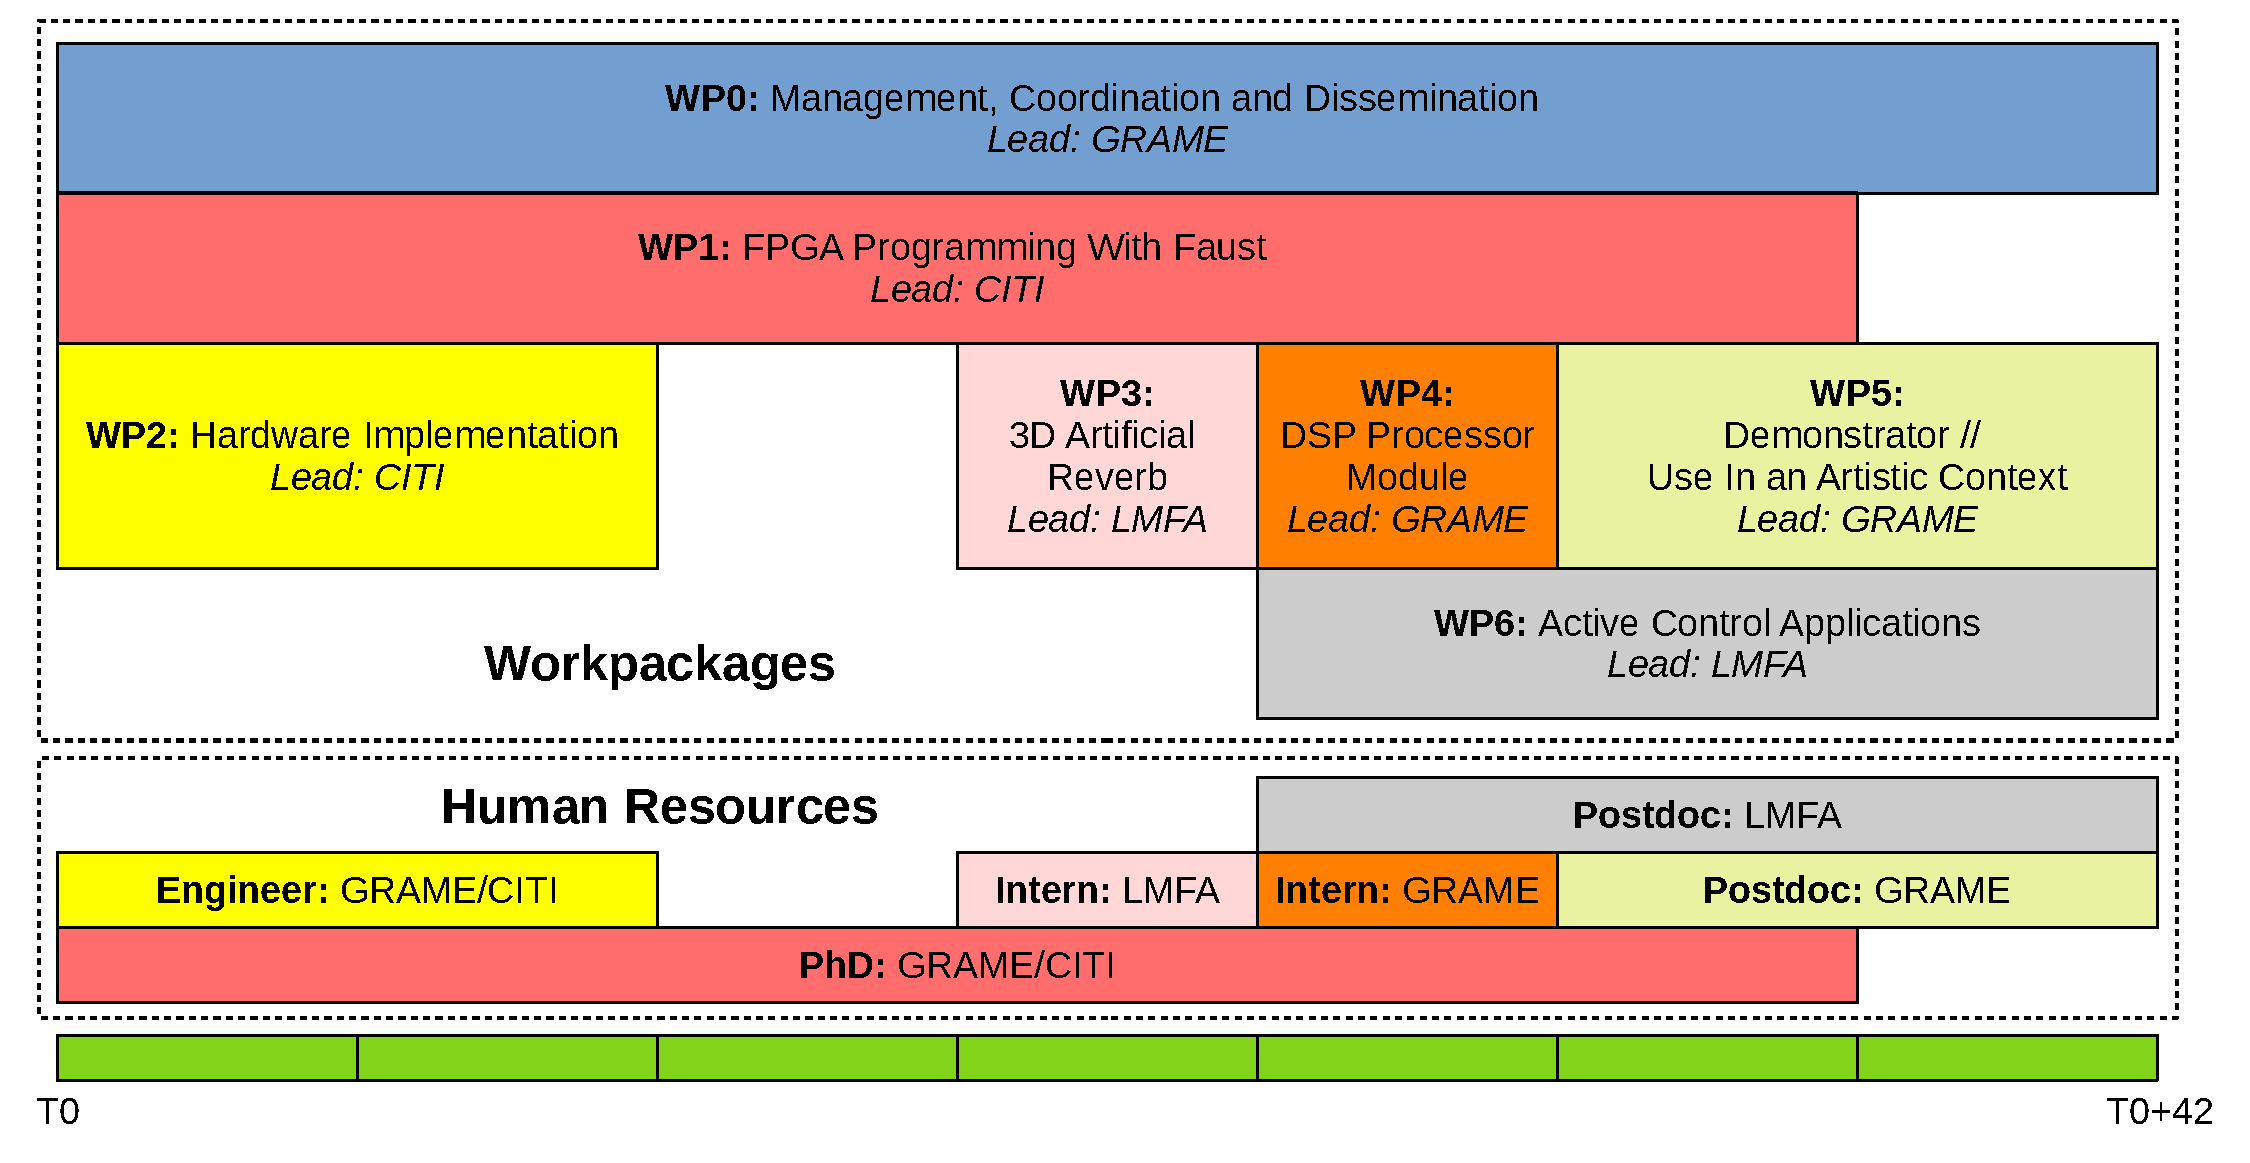
\includegraphics[width=\columnwidth]{img/wp}
  \caption{\PP{} project organization and planning.}
  \label{fig:wp}
\end{figure}

\paragraph{Human Resources}

In addition to the permanent lab members working on the project, one PhD thesis, one postdoc of one year, one postdoc of a year and a half, two 6 months Masters level internships, and one man-year of advanced engineer are foreseen (see Figure~\ref{fig:wp}). The PhD will be dedicated to modify the \F{} compiler to generate efficient FPGA IPs for real-time audio signal processing applications. One of the main challenge will be related to adding fixed-point support to the code generated by \F{} through the use of FloPoCo. The man-year of engineer at CITI will be centered around the development of the FPGA-based multichannel audio signal processor hardware platform that will be used during the next steps of the project. The masters internship at LMFA will consist in using the tools developed during the first year and half of the project to implement a multichannel artificial reverberation system in the LMFA's sound spatialization system. This will serve as a prototype for a larger system that could be used in concert halls in the framework of professional music productions. The Masters internship at GRAME-CNCM will imply the development of an audio effect/sound synthesizer module based on the platform developed in the previous steps of the project and programmable at a high level in \F{}. The postdoc at LMFA will focus on using the platform developed in the previous steps in the context of active control of room acoustics, digital lutherie, and other fields related to audio/acoustics. Finally, the postdoc (who will have a composer/artist profile) at GRAME-CNCM will apply the technologies developed throughout the project in a musical context.

\paragraph{Project Organization}

The project is organized in 6 workpackages for a total of 42 months, as detailed in Figure~\ref{fig:wp}. \textit{WP0} deals with management, coordination and dissemination. \textit{WP1} is the heart of the project and the main focus of the PhD. It will deal with adapting the \F{} compiler to generate ready-to-use efficient FPGA IPs. \textit{WP2} will begin at the same time as \textit{WP1} and will focus on implementing the hardware platform (a multichannel FPGA-based audio processor) that will be used throughout the project. \textit{WP3} will leverage the results from \textit{WP1} and \textit{WP2} to implement a spatial reverberation system in the LMFA sound spatialization system that will benefit directly from the computational power of the FPGA. % RM: am I right to say that? Does it have a more official name?
\textit{WP4} will focus on the development of a hardware and software platform for high efficiency and ultra-low-latency audio signal processing and synthesis. This platform will be controllable through a user interface as well as standard communication protocols used in the field of music (i.e., MIDI, OSC, etc.).
\textit{WP5} will involve an artist/composer/postdoc who will adapt/use/abuse the technology developed in the previous workpackages to create a musical piece that will be produced with the help of GRAME-CNCM's production department. % RM: yes? no? possible? bad idea?
Finally, \textit{WP6} will apply the platform developed in \textit{WP1} and \textit{WP2} to acoustics active control. The 2 postdocs linkeds to \textit{WP5} and \textit{WP6} will be led to collaborate. 

\paragraph{Budget (à la grosse louche)}

% RM: I think an important factor here to take into consideration is the equipment budget. Designing the hardware platform for the project (FPGA + multichannel audio ADC/DAC) will certainly have some cost but what if we wanted to buy speakers to implement a large scale sound spatialisation system like Stanford's grail, etc.?

% PL: At LMFA we have an array of 22.2 loudspeakers + spares ready to use...

% RM: Yes, but wouldn't it be nice to have a big one that we can move around in concert halls, etc. ? :)

J'ai mis l'ingé Citi/Grame dans le budget Citi, j'ai mis des chiffres au hasard pour l'équipement (à discuter). Attention, on a un pb avec le taux de précarité (cf dernière page), j'ai du gonfler artificiellement la participation des permanents de chaque institution, et on est toujours au dessus des 30\%, il faut regarder serieusement, je ne sais pas si c'est toujours une contrainte de l'ANR. 
\begin{center}\small
  \begin{spreadtab}{{tabular}{|c|c|c|c||c|}}
\hline
 &@Insa-Lyon & @Centrale-Lyon  & @Grame &   @Total \\ 
 & @Citi & @LMFA & & \\ 
 & @(rate 100\%) & @(100\%) &   @(rate 100\%) &  @(k\euro)\\ \hline \hline
@Man Month ANR & 48 & 18  & 12 & \\ \hline
% calcul Insa 36 mois PhD + 12 mois ingé confirmé 36*3083+12*3924
% clacul Centrale fait avec les cout insa 18**3924
% calcul Grame fait avec les cout insa 12*3924 + 12*554
@Staff (k\euro)   & 158 & 71 & 54 & sum(b5:d5) \\ \hline
@Equipment  (k\euro)   &  5 &  10  & 10 &sum(b6:d6) \\  \hline
@Travel  (k\euro)    &  20 & 50  &50  & sum(b7:d7)\\  \hline
@Management  (k\euro)    &  5 & 5  & 15  & sum(b8:d8) \\
\hline\hline
@Total requested (k\euro)     & sum(b5:b8)  & sum(c5:c8)    & sum(d5:d8)  & sum(e5:e8)  \\ \hline
\end{spreadtab}

\end{center}

\section*{Project Impact and Benefits}

Audio DSP is used everywhere is nowadays life (e.g., smartphones, TVs, cars, tablets, computers, musical instruments, speakers, etc.). Computational power and low-latency are probably the most important technical factors when it comes to these types of systems. FPGAs can help take this field to a new level. This is only possible if this type of platform is easily accessible to non-FPGA engineers. We believe that \PP{} has the potential to revolutionize the field of real-time audio DSP in the same way than Arduinos disrupted the world of prototyping and engineering. % RM: too much? :)
Possibilities unveiled by these developments will impact a wide range of fields and could lead to plethora of technological and industrial applications to design concert halls of a new kind, suppress noise in a car's passenger compartment, diminish vibrations in airplane jet engines, improve existing digital musical instrument technologies, etc. 

\bibliographystyle{plain}
\bibliography{main,pierre}

% \newpage
% \section{A enlever avant de soumettre: Taux de précarité (pas vérifié la formule 2018)}
% {Man month repartition per  partner }
% 
% \begin{spreadtab}{{tabular}{|c||p{2.4cm}|p{2cm}|p{2.7cm}|p{2.5cm}||p{1cm}|}}
% \hline
% @Institution &
% @permanent
%  (institution) &
% @permanent 
%  (ANR) &
% @Non-permanent
%  (ANR) &
% @PhD thesis and internship &
% @Total
%  \\ \hline \hline
% @Insa Citi 	& 24 	& 	&  12	& 36 & sum(b2:e2) \\
% \hline
% @Centrale LMFA  	&  12	& 	&  18	&    & sum(b3:e3) \\
% \hline
% @Grame	&  24	&   	& 12	&  & sum(b4:e4) \\
% \hline \hline 
% @Total 	&  sum(b2:b4)	&  sum(c2:c4)	& sum(d2:d4) & sum(e2:e4)  &  sum(b7:e4)\\
% \hline
% \multicolumn{6}{|l|}{\em taux de précarité (<<d5>>/(<<b5>>+<<c5>>+<<d5>>)) :  :={round(d5/sum(b5:d5),3)}} \\
% \hline
% \end{spreadtab}



\end{document}
